% MNS project 2010 report
%
% Luís Francisco Seoane Iglesias
% Mirko Dietrich - mirko.dietrich -AT- bccn-berlin -DOT- de
% 

\documentclass[a4paper,12pt,oneside]{article}

\usepackage[utf8x]{inputenc}
\usepackage{amsmath}
\usepackage{cite}
\usepackage{graphicx}
\usepackage{epsfig}
%\usepackage{html}
% Line spacing
\usepackage{setspace}

%\sloppy

% typeset physical units
\newcommand{\unit}[1]{\ensuremath{\, \mathrm{#1}}}

\begin{document}

\begin{titlepage}
\begin{center}
\begin{spacing}{2}
{\huge\bf Spike-timing-dependent plasticity} \\
\end{spacing}
\Large
Project report \\
\vfill
\normalsize
\today \\
\vspace{5em}
Models of Neural Systems WS 09/10 \\
\vspace{1em}
Luís Francisco Seoane Iglesias \\
Mirko Dietrich \\
\vspace{1em}
Bernstein Center for Computational Neuroscience Berlin
\end{center}
\end{titlepage}

\tableofcontents

\newpage

%%%%%%%%%%%%%%%%%%%%%%%%%%%%%%%%%%%%%%%%%%%%%%%%%%%%%%%%%%%%%%%%%%%%%%%%%%%%%%%
\section{Introduction}

While the Hebbian learning rule says that \textit{cells that fire
  together, wire together} the Spike-timing-dependent plasticity
theory states more precisely by describing a relation between synapse
plasticity and the time between pre- and post-synaptic spikes. It finds
when a presynaptic precedes a post-synaptic spike the corresponding
synapse connectivity is strengthened. On the other hand when a
presynaptic follows a post-synaptic action potential the efficacy of
synapse transmission decreases.\cite{Song:2000}

%%%%%%%%%%%%%%%%%%%%%%%%%%%%%%%%%%%%%%%%%%%%%%%%%%%%%%%%%%%%%%%%%%%%%%%%%%%%%%%
\section{Methods}

We modelled a neuron with a number of inhibitory and excitatory
synapses connected to it. The neuron's voltage is calculated using a
modified integrate-and-fire model. Synaptic conductances $g_{in}$ and
$g_{ex}$ change with time:

\[
\tau_m \frac{dV}{dt} = V_{rest} – V + g_{ex}(t)(E_{ex} – V) + g_{in}(t)(E_{in} – V). 
\]

A post-synaptic action potential is triggered when the cell's resting
potential reaches a threshold of $-54\unit{mV}$. Afterwards the
voltage is reset to $-60\unit{mV}$.

Whenever a presynaptic spike arrives the synapse conductance is changed:

\[
g_{ex}(t) \rightarrow g_{ex}(t)+\bar{g}_{a}, 
\]
for excitatory connections and: 
\[
g_{in}(t) \rightarrow g_{in}(t)+\bar{g}_{in}
\]
for inhibitory. 

If no presynaptic spike occurs the conductance decays exponentially:

\[
\tau_{ex} \frac{dg_{ex}}{dt} = -g_{ex},\hspace{1em} \tau_{in} \frac{dg_{in}}{dt} = -g_{in}. 
\]

	To model the Hebbian learning, two functions are introduced: $P(t)$, which carries information about the reward a synapses would receive if it makes the post-synaptic dendrite fire; and $M(t)$, which says which would be the penalty if an action potential arrives to the synapse after the post-synaptic dendrite has fired. 
	
	Every time that the post-synaptic neuron fires an action potential, the $M(t)$ function is decreased by an amount $A_-$, then $M(t)$ exponentially decays to zero. If any presynaptic neuron would fire during this decay, it means: out of time, it would receive a penalty proportional to $M$ by modifying its connectivity: 
		\begin{eqnarray} 
			\bar{g}_a &\rightarrow& \bar{g}_a + M(t)\bar{g}_{max}. 
		\end{eqnarray}
		
	With the same idea, each time that a presynaptic neuron fires an action potential, $P(t)$ is increased an amount $A_+$ and the decays exponentially toward zero. If this action potential would contribute to the firing of the post-synaptic neuron, eliciting an action potential in it during the time-window delimited by the decay of $P(t)$; then the synapse would receive a reward proportional to $P(t)$:
		\begin{eqnarray} 
			\bar{g}_a &\rightarrow& \bar{g}_a + P(t)\bar{g}_{max}. 
		\end{eqnarray}

	The range for $\bar{g}_a$ is $[0,g_{max}]$, which would avoid infinite increase or decrease of these quantities. 
	
	\begin{figure}[h]
		\centering
		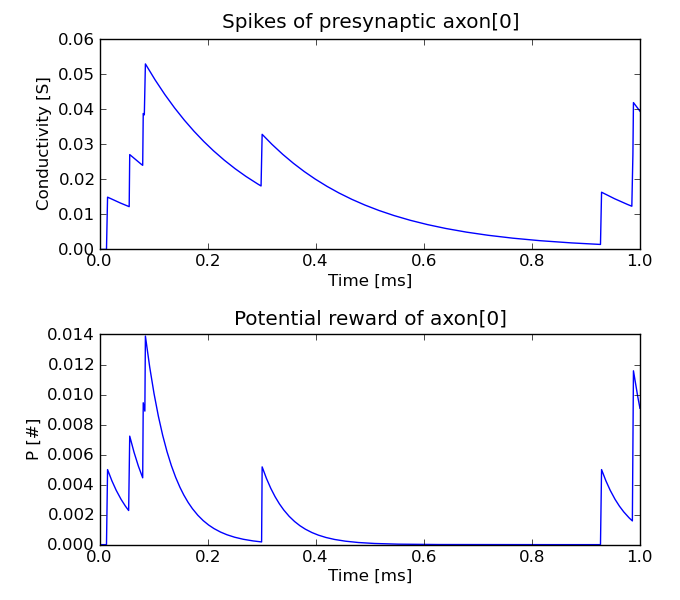
\includegraphics[width=0.8\textwidth]{graphics/demo/fig01}
		\caption{ }
		\label{fig:2.2}
	\end{figure}
	

\subsection{Parameters}

The following parameters were used for the simulation:

\begin{align*}
  \tau_m &= 20\unit{ms} \\
  V_{rest} &= -70\unit{mV} \\
  E_{ex} &= 0\unit{mV} \\
  E_{in} &= -70\unit{mV} \\
  \tau_{ex} = \tau_{in} &= 5\unit{ms} \\
  \bar{g}_{in} &= 0.05 \\
  \bar{g}_{max} &= 0.0015
\end{align*}

%%%%%%%%%%%%%%%%%%%%%%%%%%%%%%%%%%%%%%%%%%%%%%%%%%%%%%%%%%%%%%%%%%%%%%%%%%%%%%%
\section{Results}

	\subsection{Balanced Excitation} 
		\label{sub:3.1}
	
		In the frame of the model, presynaptic neurons would compete with each other to drive the behavior of the post-synaptic one. This competition is reflected in the variation of the connectivity of the neurons and should lead to a stable distribution of the weights $\bar{g}_a$. 
		
		We implemented an experiment in which a population of $200$ inhibitory and $1000$ excitatory presynaptic neurons would connect to a dendrite. The inhibitory neurons would spike with a frequency of 10Hz and the excitatory ones would spike with frequencies in the range $f=[10,40]$ Hz for many realizations of the experiment. Our aim was to study the steady distribution of $\bar{g}_a/\bar{g}_{max}$, but the convergence time showed up to be quite large --even with soft convergence criteria-- so here are presented only approximate results. 
		
		In figures \ref{fig:T5.01}a, \ref{fig:T5.01}a, are \ref{fig:T5.01}c are represented many captures of the distribution of weights for a firing rate of $40$ Hz in the presynaptic neurons, using a time step of $0.01$ ms in the simulation. After the data given in the paper \cite{paper} it was expected that such a simulation for $f=40$ Hz would lead to a distribution of $\bar{g}_a/\bar{g}_{max}$ in which the neurons would tend to the extreme values ($\bar{g}_a/\bar{g}_{max}=0$ or $\bar{g}_a/\bar{g}_{max}=1$), being dominant those neurons with low connectivity. We see in the figures how this tendency is reproduced. 
		
		Notwithstanding that, we have also found that this behavior depends in a great manner on the parameters of the simulation. In figures \ref{fig:T5.01}d, \ref{fig:T5.01}e and \ref{fig:T5.01}f is reproduced the same experiment with a time step of $0.1$ ms and the expected outcome disappears. In any case, it should be pointed out that none of these distribution is stable and that changes greater that $1\%$ happened in the value of $\bar{g}_a$ for at least one of the synapses. 
		
		\begin{figure}
			\begin{picture}(70,400)
				\put(0,300){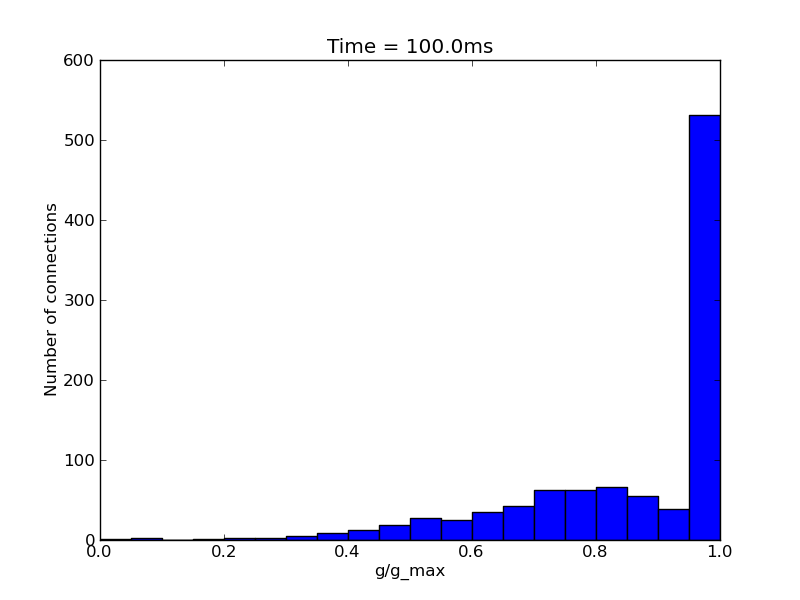
\includegraphics[width=0.5\textwidth]{graphics/task5/40/100}}
				\put(200,300){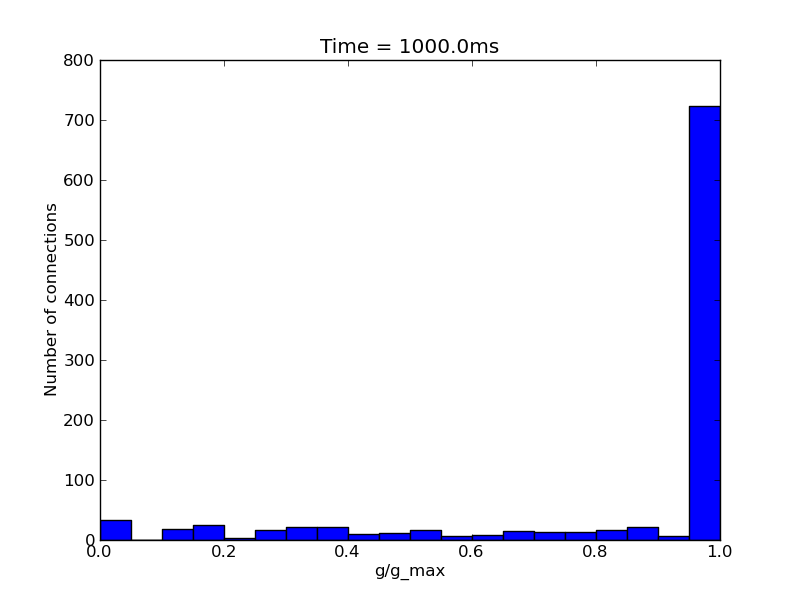
\includegraphics[width=0.5\textwidth]{graphics/task5/40/1000}} 
				\put(0,150){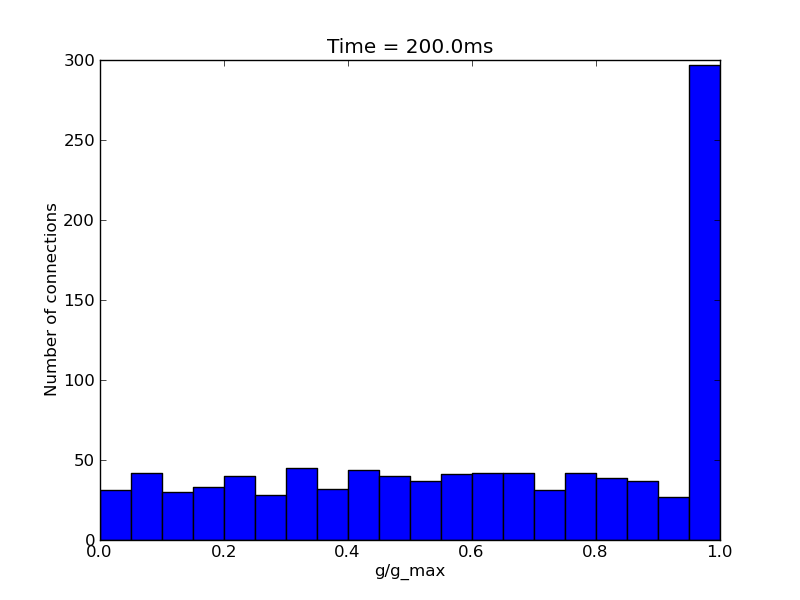
\includegraphics[width=0.5\textwidth]{graphics/task5/40/200}}
				\put(200,150){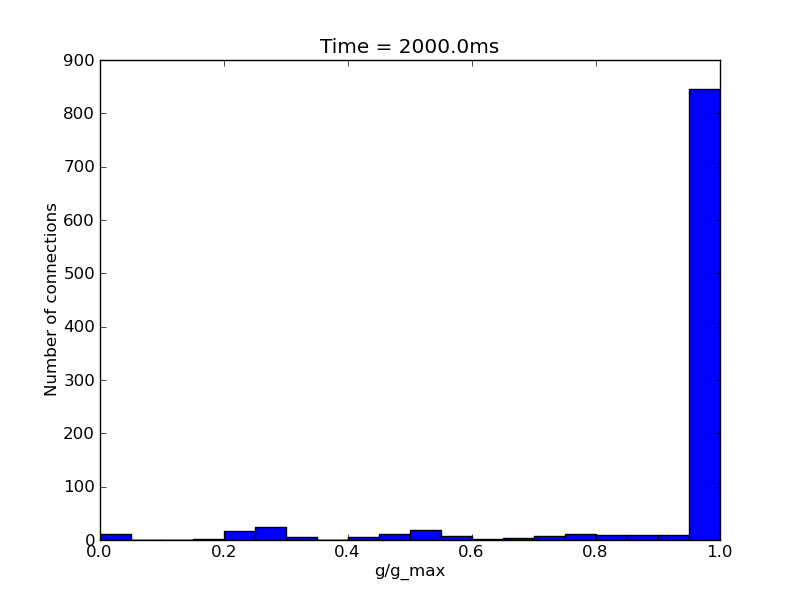
\includegraphics[width=0.5\textwidth]{graphics/task5/40/2000}}
				\put(0,0){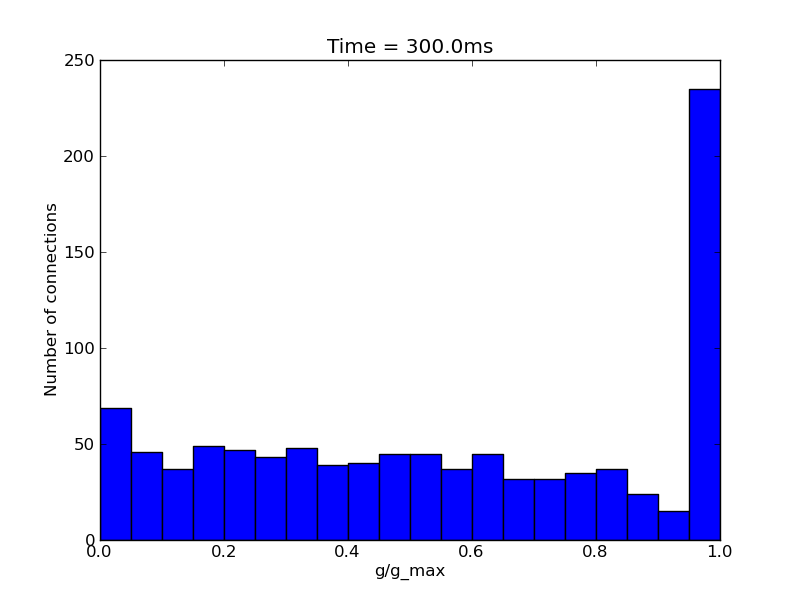
\includegraphics[width=0.5\textwidth]{graphics/task5/40/300}}
				\put(200,0){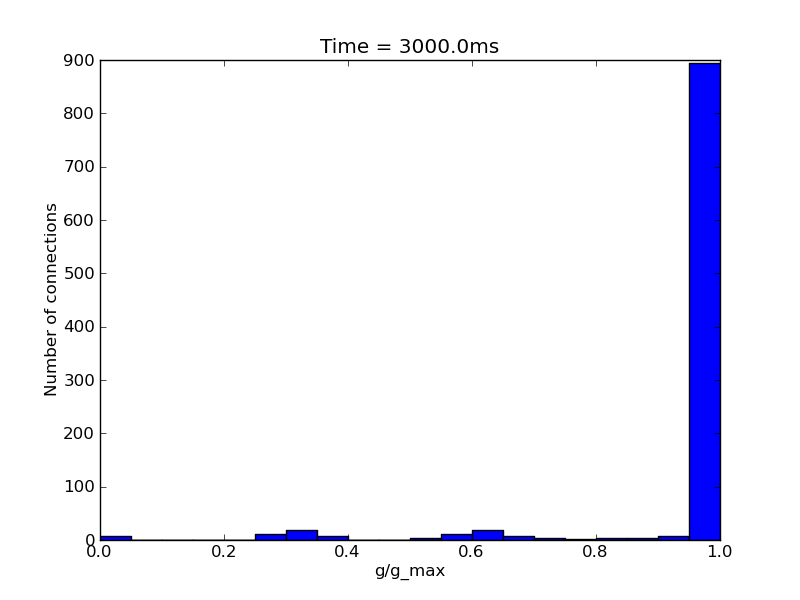
\includegraphics[width=0.5\textwidth]{graphics/task5/40/3000}}
				\put(0,430){a)}
				\put(200,430){d)}
				\put(0,280){b)}
				\put(200,280){e)}
				\put(0,130){c)}
				\put(200,130){f)}
			\end{picture}
			\caption{}
                  		\label{fig:T5.01}
		\end{figure}
		
		In figures \ref{fig:T5.02}a, \ref{fig:T5.02}b and \ref{fig:T5.02}c is presented anther example of the experiment, in this case for $f=10Hz$. Again, from the paper it was expected that the distribution would center in the extremes ($\bar{g}_a/\bar{g}_{max}=0$ or $\bar{g}_a/\bar{g}_{max}=1$), being $\bar{g}_a/\bar{g}_{max}=1$ largely dominant. From the non-steady distribution plotted in these figures, we can not expect that this would happen. Again, a huge different happens for very close different values of the time step of the simulation. 
		
		\begin{figure}
			\begin{picture}(70,400)
				\put(0,300){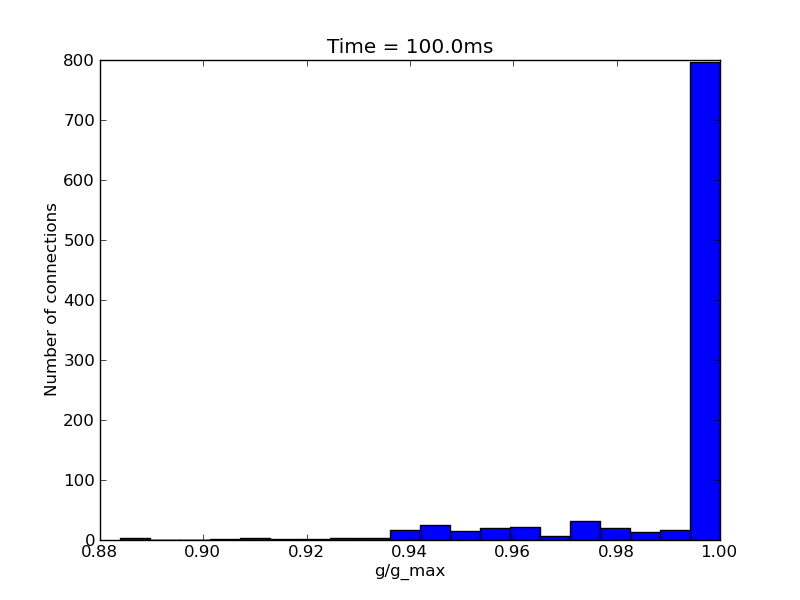
\includegraphics[width=0.5\textwidth]{graphics/task5/10/100}}
				\put(200,300){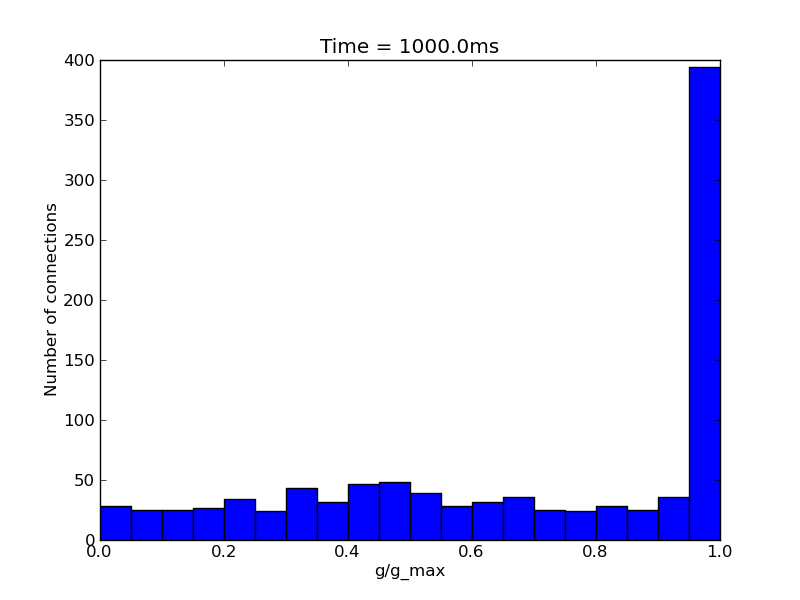
\includegraphics[width=0.5\textwidth]{graphics/task5/10/1000_}} 
				\put(0,150){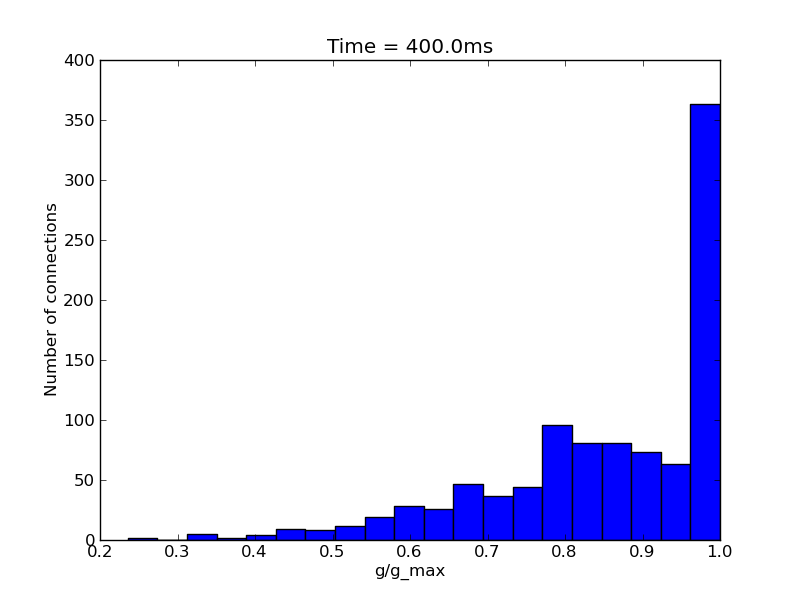
\includegraphics[width=0.5\textwidth]{graphics/task5/10/400}}
				\put(200,150){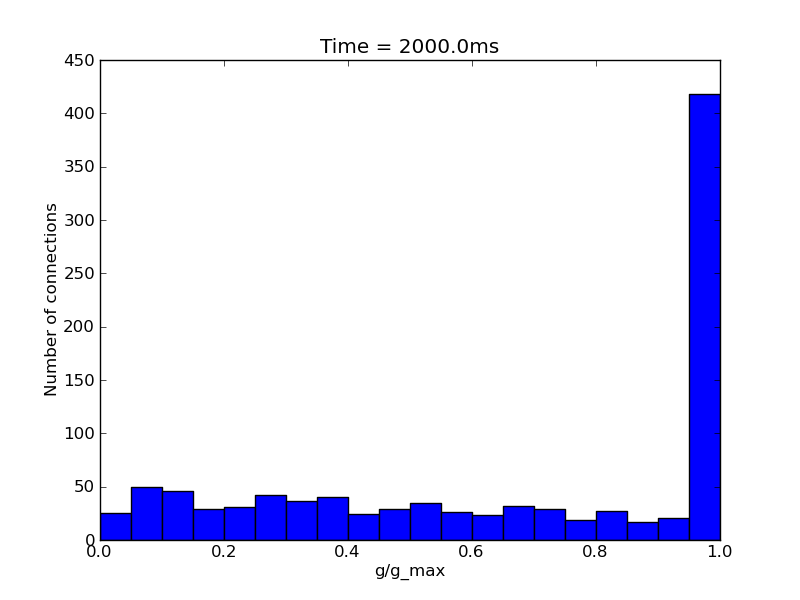
\includegraphics[width=0.5\textwidth]{graphics/task5/10/2000_}}
				\put(0,0){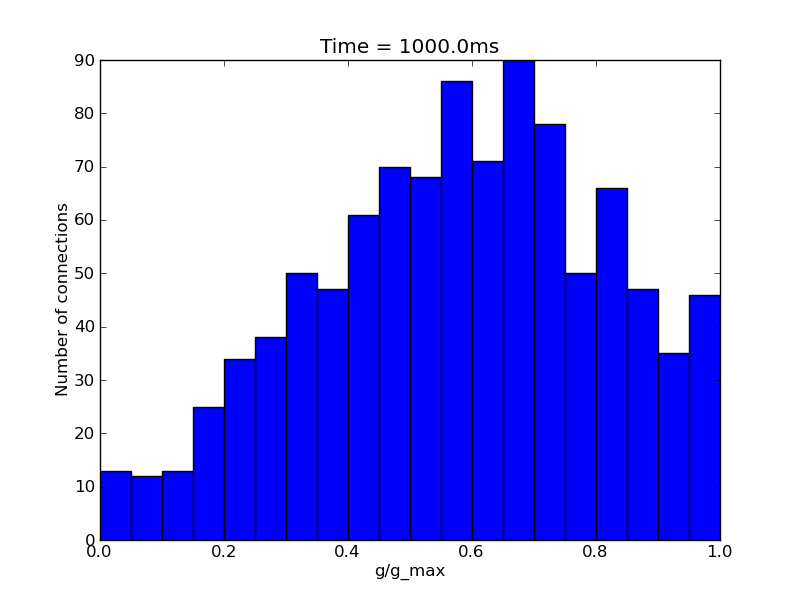
\includegraphics[width=0.5\textwidth]{graphics/task5/10/1000}}
				\put(200,0){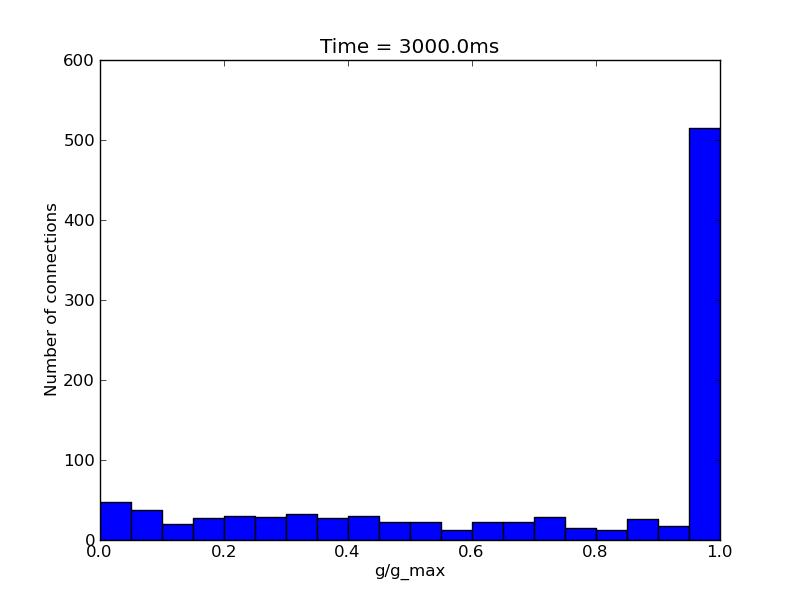
\includegraphics[width=0.5\textwidth]{graphics/task5/10/3000_}}
				\put(0,430){a)}
				\put(200,430){d)}
				\put(0,280){b)}
				\put(200,280){e)}
				\put(0,130){c)}
				\put(200,130){f)}
			\end{picture}
			\caption{}
                  		\label{fig:T5.02}
		\end{figure}
		
	\subsection{Latency Reduction} 
	
		An experiment was carried out to test the model when a the presynaptic neurons presented some latency. To do so, again with the $200$ inhibitory and $1000$ excitatory neurons, the input from excitatory neurons was set to be silent except for bursts of bursts 
		

%%%%%%%%%%%%%%%%%%%%%%%%%%%%%%%%%%%%%%%%%%%%%%%%%%%%%%%%%%%%%%%%%%%%%%%%%%%%%%%
\section{Discussion}

	\subsection{Balanced Excitation} 
	
		The main problem encountered to implement this experiment was the great dependence of the outcome on the parameters of the simulation. More precisely, the great different of the result depending on the time step made it impossible to obtain reliable data. In the paper in which this work is based there are not provided any technical detail related to this point, thus it was not possible for us to reproduce the figures. 
		
		As an example of this criticality, already pointed out in subsection \ref{sub:3.1}, is that a large time step would sweep away the expected behavior, while with a slightly smaller time step the tendency can be at least observed, though the convergence takes more than it was possible for us to simulate the system. Smaller time steps would lead to increasing converging times, and eventually a very small time step would yield a spike probability ($f\cdot\Delta T$) so low that it would not be observed any spike of the post-synaptic neuron. 
		
		In this task we were also asked to plot the Coefficient of variation (CV) of the post-synaptic spike train and the frequency at which this post-synaptic neuron would spike, both when the stable distribution $\bar{g}_a/\bar{g}_{max}$ had been achieved. Since We did not achieve this stability in any case we simulated, such representations were not made. 

%%%%%%%%%%%%%%%%%%%%%%%%%%%%%%%%%%%%%%%%%%%%%%%%%%%%%%%%%%%%%%%%%%%%%%%%%%%%%%%
\section{Contributions}
Describe who did what (programming, writing of the report, figures,...)

%%%%%%%%%%%%%%%%%%%%%%%%%%%%%%%%%%%%%%%%%%%%%%%%%%%%%%%%%%%%%%%%%%%%%%%%%%%%%%%
\newpage
\bibliographystyle{plain}
\bibliography{report}

\end{document}
